\documentclass[11pt,a4paper]{article}
\usepackage[margin=2.5cm]{geometry}
\usepackage{graphicx}
\usepackage{booktabs}
\usepackage{amsmath}
\usepackage{amssymb}
\usepackage{hyperref}
\usepackage{parskip}
\usepackage{microtype}
\usepackage[T1]{fontenc}
\usepackage{lmodern}

\graphicspath{{./}{../multihead-outputs/}{../../output/stance/}}

\title{\textbf{LLM Disagreement on Central Bank Stance}\\[0.4em]
       \large Method, Evidence, and What It Means for the Thesis}
\author{Samuel Fraley \\ BSE Thesis 2025--2026}
\date{\today}

\begin{document}
\maketitle
\tableofcontents
\vspace{1em}

% ─────────────────────────────────────────────────────────────────────────────
\section{Research Questions}

The thesis asks whether central bank communication shocks spill over into
institutions and financial markets, and whether language models agree on those
shocks. Four sub-questions motivate this note:

\begin{enumerate}
  \item Do different LLMs classify Fed, ECB, and BoE communication differently,
        and where does disagreement arise?
  \item Does the choice of LLM meaningfully affect the estimated communication
        shocks and spillover results?
  \item Do communication shocks from one central bank predict changes in tone
        from other central banks?
  \item Do these communication shocks generate asymmetric cross-border market
        reactions?
\end{enumerate}

This note addresses \textbf{RQ1 and RQ2} in detail. RQ3 and RQ4 remain
the subject of ongoing VAR estimation and are flagged at the end.

% ─────────────────────────────────────────────────────────────────────────────
\section{Scoring Pipeline}

We classify approximately 5,000 central bank speech chunks (Fed, ECB, BoE)
using four large language models: \textbf{Llama 3.3}, \textbf{DeepSeek V3},
\textbf{Qwen 2.5 72B}, and \textbf{Mistral Large}. Each chunk is labelled on
a five-point scale:

\begin{center}
\textit{dovish} $\;\longrightarrow\;$
\textit{mostly dovish} $\;\longrightarrow\;$
\textit{neutral} $\;\longrightarrow\;$
\textit{mostly hawkish} $\;\longrightarrow\;$
\textit{hawkish}
\end{center}

Labels are converted to a numeric score ($-1, -0.5, 0, +0.5, +1$) and
aggregated to meeting-level averages. Rather than treating disagreement between
models as a nuisance to be averaged away, this note investigates its source ---
because if models disagree systematically, that structure is information.

% ─────────────────────────────────────────────────────────────────────────────
\section{Do the LLMs Agree?}

\subsection{Inter-rater agreement}

We measure agreement using Cohen's $\kappa$ on all pairwise model combinations.
A hierarchical decomposition separates two sources of disagreement:

\begin{itemize}
  \item \textbf{Stancing disagreement} ($\kappa_\text{stanced} = 0.56$--$0.69$):
        whether a chunk is directional (hawkish or dovish) vs.\ neutral.
  \item \textbf{Direction disagreement} ($\kappa_\text{direction} = 0.88$--$0.98$):
        given both models call a chunk directional, do they agree on the direction?
\end{itemize}

The takeaway is stark: \textbf{models agree almost perfectly on direction but
disagree substantially on whether to call a chunk stanced at all.} The
disagreement is not about which way the wind is blowing --- it is about whether
there is any wind.

\begin{figure}[h!]
  \centering
  \includegraphics[width=0.85\textwidth]{agreement_kappa_hierarchical.png}
  \caption{Hierarchical $\kappa$ decomposition. Direction $\kappa$ is
           near-perfect across all model pairs; stancing $\kappa$ is moderate.}
\end{figure}

\subsection{Disagreement over time}

Figure~\ref{fig:disagreement_ts} shows disagreement between models across
calendar time. Spikes correspond to high-uncertainty meetings (e.g.\ policy
pivots, GFC aftermath, 2022 tightening cycle), consistent with the hypothesis
that disagreement is higher when the text itself is harder to read.

\begin{figure}[h!]
  \centering
  \includegraphics[width=\textwidth]{timeseries_disagreement_llama33_deepseekv3_qwen25_72b_mistrallarge_or.png}
  \caption{Pairwise model disagreement over time. Shaded bands show
           inter-model range.}
  \label{fig:disagreement_ts}
\end{figure}

% ─────────────────────────────────────────────────────────────────────────────
\section{What Drives Disagreement? Four Null Results}

Before testing a mechanistic model, we ruled out four surface-level explanations.

\begin{center}
\renewcommand{\arraystretch}{1.4}
\begin{tabular}{lll}
\toprule
\textbf{Hypothesis} & \textbf{Test} & \textbf{Result} \\
\midrule
Chunks are semantically ambiguous & Embedding cosine AUC & 0.50 (chance) \\
Chunks contain more hedging language & Hedge density ratio & $1.07\times$ (n.s.) \\
Chunks use conditional syntax & Modal / policy arc count & $\approx 0$ effect \\
Chunk reverses prior meeting direction & Meeting context AUC & 0.52 (chance) \\
\bottomrule
\end{tabular}
\end{center}

None of these features predict whether a chunk will be disputed. Disagreement
is not explained by the text being vague, hedged, conditional, or surprising
relative to recent meetings. This pushed us toward a token-level investigation.

% ─────────────────────────────────────────────────────────────────────────────
\section{Same Signals, Different Weights}

\subsection{Phrase masking}

We ran a two-pass experiment on 100 high-disagreement chunks. First, each
model identified 3--8 key phrases (exact substrings) that drove its
classification. Then we masked each phrase in turn and asked all four models
to re-score.

\textbf{59 of 100 disagreements resolved when a single phrase was masked},
confirming disagreement is localised to specific spans --- not spread across
the whole chunk.

\subsection{Chain-of-thought reasoning}

We prompted models to reason step-by-step before labelling: list hawkish
signals, list dovish signals, explain the weighing, then label. Signal overlap
between models was measured with word-level Jaccard similarity:

\begin{center}
\begin{tabular}{lc}
\toprule
\textbf{Signal type} & \textbf{Jaccard overlap} \\
\midrule
Hawkish signals & 0.656 \\
Dovish signals  & 0.396 \\
\bottomrule
\end{tabular}
\end{center}

Models identify largely the same hawkish signals but diverge more on dovish
ones. Crucially, high overlap coexists with high disagreement: there is no
correlation between Jaccard overlap and disagreement magnitude. \textbf{Models
are listing the same phrases and still disagreeing on the label.} The
disagreement is about how much weight to give each signal --- not about
perceiving different signals.

% ─────────────────────────────────────────────────────────────────────────────
\section{The Multi-Head Model}

\subsection{What problem are we solving?}

Phrase masking and CoT tell us disagreement is about signal weighting. But
``weighting'' is vague. We want a precise, mechanistic answer: \emph{given
the same internal representation of a text, do the models apply different
decision rules?} The multi-head model is designed to answer exactly this.

\subsection{The shared encoder}

We use \textbf{DeBERTa-v3-base}, a transformer encoder pretrained on a large
text corpus. Think of it as a sophisticated reading-comprehension model that
compresses any text passage into a \textbf{768-number summary vector} --- a
dense representation capturing the monetary policy content of the text. This
vector is called the \texttt{[CLS]} embedding. The model has been exposed to
hundreds of billions of words and already ``knows'' what words like
\textit{accommodation}, \textit{tightening}, and \textit{transmitted} signal in
a central banking context.

\subsection{The four classification heads}

Each LLM gets its own \textbf{decision rule}: a matrix of learned weights with
5 rows (one per stance label) and 768 columns (one per dimension of the summary
vector). To predict a label, the head multiplies the 768-number summary by its
weight matrix and picks the stance with the highest score.

\begin{equation*}
\text{logits}_k = W_k \cdot \mathbf{c} \qquad
W_k \in \mathbb{R}^{5 \times 768}, \quad
\mathbf{c} \in \mathbb{R}^{768}
\end{equation*}

This is a \textbf{linear projection} --- the simplest possible mapping from the
shared representation to a label. There are no hidden layers, no nonlinearities.
The head is literally a single matrix multiplication. This matters because we
can inspect the weight matrix directly and compare it across models.

\subsection{Why train all four heads together?}

Training all four heads simultaneously on the same encoder forces the
768-number summary to contain whatever all four models need to make their
decisions. If Llama needs \textit{accommodation} to be salient to label a
chunk dovish, and Qwen needs \textit{tightening} to label a different chunk
hawkish, the encoder learns to represent both --- because it must satisfy all
four heads at once. The shared encoder is a bottleneck that extracts a
universal representation of monetary policy language.

In the first training epoch, the encoder is frozen and only the heads are
updated. This lets each head learn to use the encoder's existing representations.
In epochs two and three, the encoder unfreezes and the whole model is fine-tuned
jointly at a low learning rate.

\subsection{Test set results}

\begin{center}
\begin{tabular}{lcc}
\toprule
\textbf{Model} & \textbf{Accuracy} & \textbf{Macro-F1} \\
\midrule
Llama 3.3       & 76.0\% & 0.519 \\
DeepSeek V3     & 83.2\% & 0.387 \\
Qwen 2.5 72B    & 87.6\% & 0.422 \\
Mistral Large   & 79.9\% & 0.533 \\
\bottomrule
\end{tabular}
\end{center}

The accuracy--F1 gap for DeepSeek and Qwen reflects their strong neutral bias:
high accuracy is achieved by predicting neutral more often, but directional
classes are missed (low F1). Llama and Mistral are more willing to commit to a
directional label, producing lower accuracy but better F1.

\begin{figure}[h!]
  \centering
  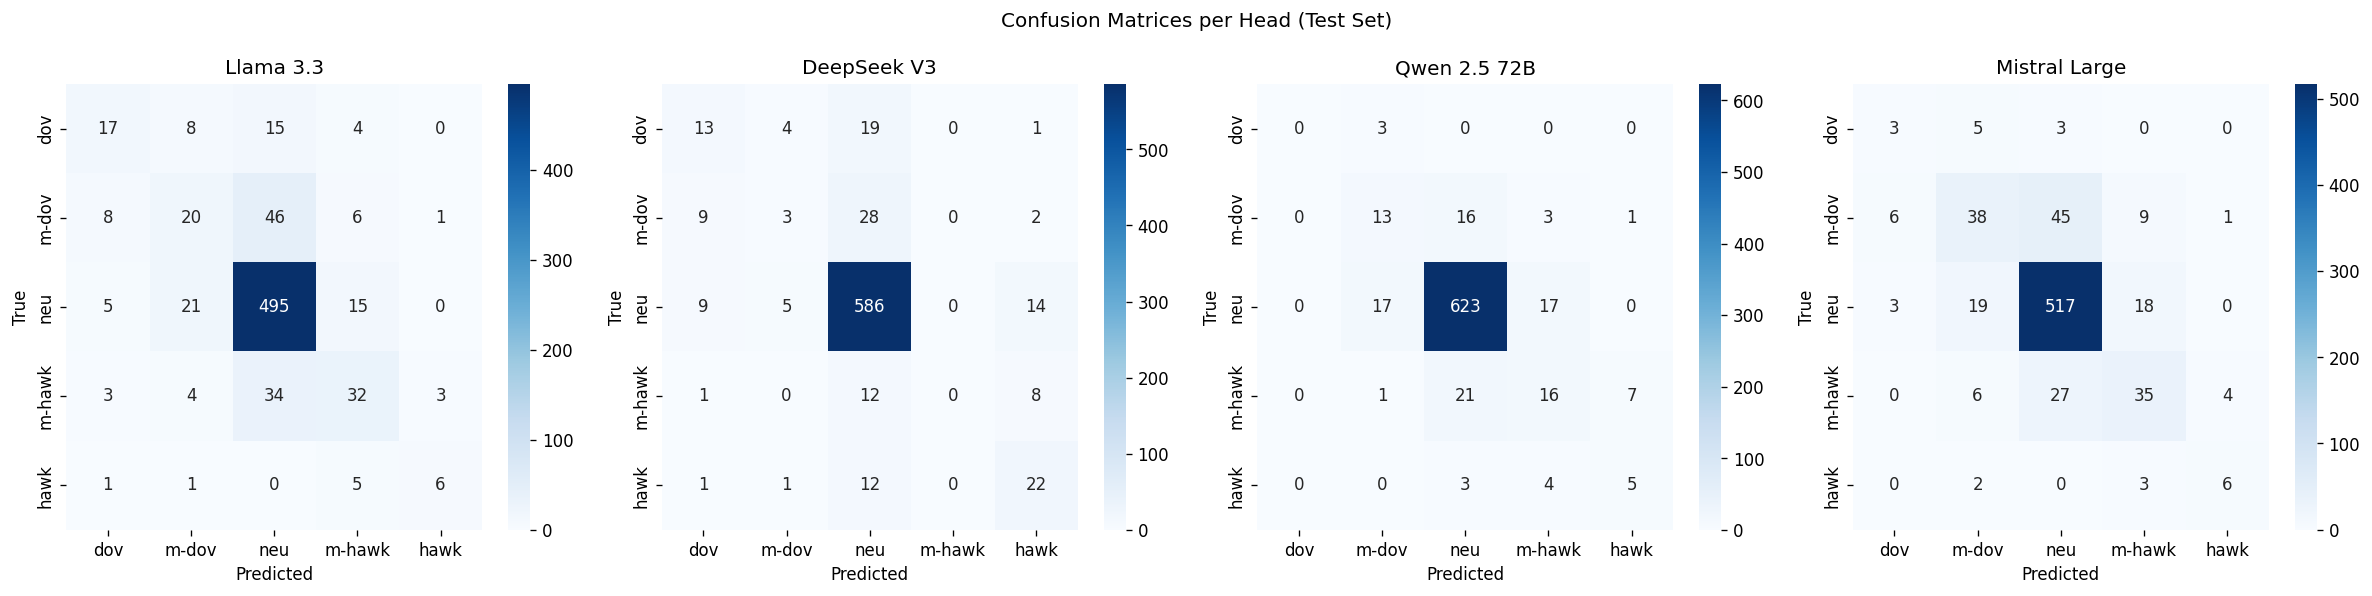
\includegraphics[width=\textwidth]{confusion_matrices.png}
  \caption{Confusion matrices per head (test set). All heads over-predict
           \textit{neutral}; Llama and Mistral make more directional calls.}
\end{figure}

% ─────────────────────────────────────────────────────────────────────────────
\section{What the Heads Learned}

\subsection{Gradient attribution: which tokens drive each head?}

For each disagreement chunk in the test set, we ask: which tokens most
influenced each head's prediction? We compute the gradient of the predicted
label's score with respect to the input word embeddings. Tokens with large
gradients caused large changes in the prediction --- they are what the head
``looked at.''

Averaging over 194 disagreement chunks, the top tokens per head are:

\begin{center}
\renewcommand{\arraystretch}{1.3}
\begin{tabular}{lllll}
\toprule
\textbf{Rank} & \textbf{Llama 3.3} & \textbf{DeepSeek V3} &
               \textbf{Qwen 2.5 72B} & \textbf{Mistral Large} \\
\midrule
1 & accommodation & accommodation & transmitted   & transmitted \\
2 & transmitted   & accommodative & accommodative & accommodative \\
3 & \textit{draghi}       & transmitted   & accommodation & accommodation \\
4 & accommodative & \textit{draghi}       & \textbf{hikes}         & \textbf{hikes} \\
5 & \textit{ecb}          & \textit{ecb}          & \textbf{tightening}    & ecb \\
\bottomrule
\end{tabular}
\end{center}

The shared core --- \textit{accommodation}, \textit{accommodative},
\textit{transmitted} --- appears in every head. The encoder has learned a
universal monetary policy signal vocabulary, and all heads perceive it. This
directly confirms the CoT finding.

The divergence is in what else each head responds to:
\begin{itemize}
  \item \textbf{Llama and DeepSeek} additionally weight \textit{entity names}:
        \textit{draghi}, \textit{ecb}. These heads are partly classifying on
        \emph{who is speaking}, not just what is being said.
  \item \textbf{Qwen and Mistral} additionally weight \textit{explicit
        directional vocabulary}: \textit{hikes}, \textit{tightening}. These heads
        are more purely lexical-stance driven.
\end{itemize}

A practical consequence: a Draghi speech using neutral language will be pulled
toward non-neutral by Llama and DeepSeek (speaker cue) but left near neutral by
Qwen and Mistral (no explicit stance word). This is a systematic disagreement
pattern that cannot be reduced to ambiguity in the text.

\begin{figure}[h!]
  \centering
  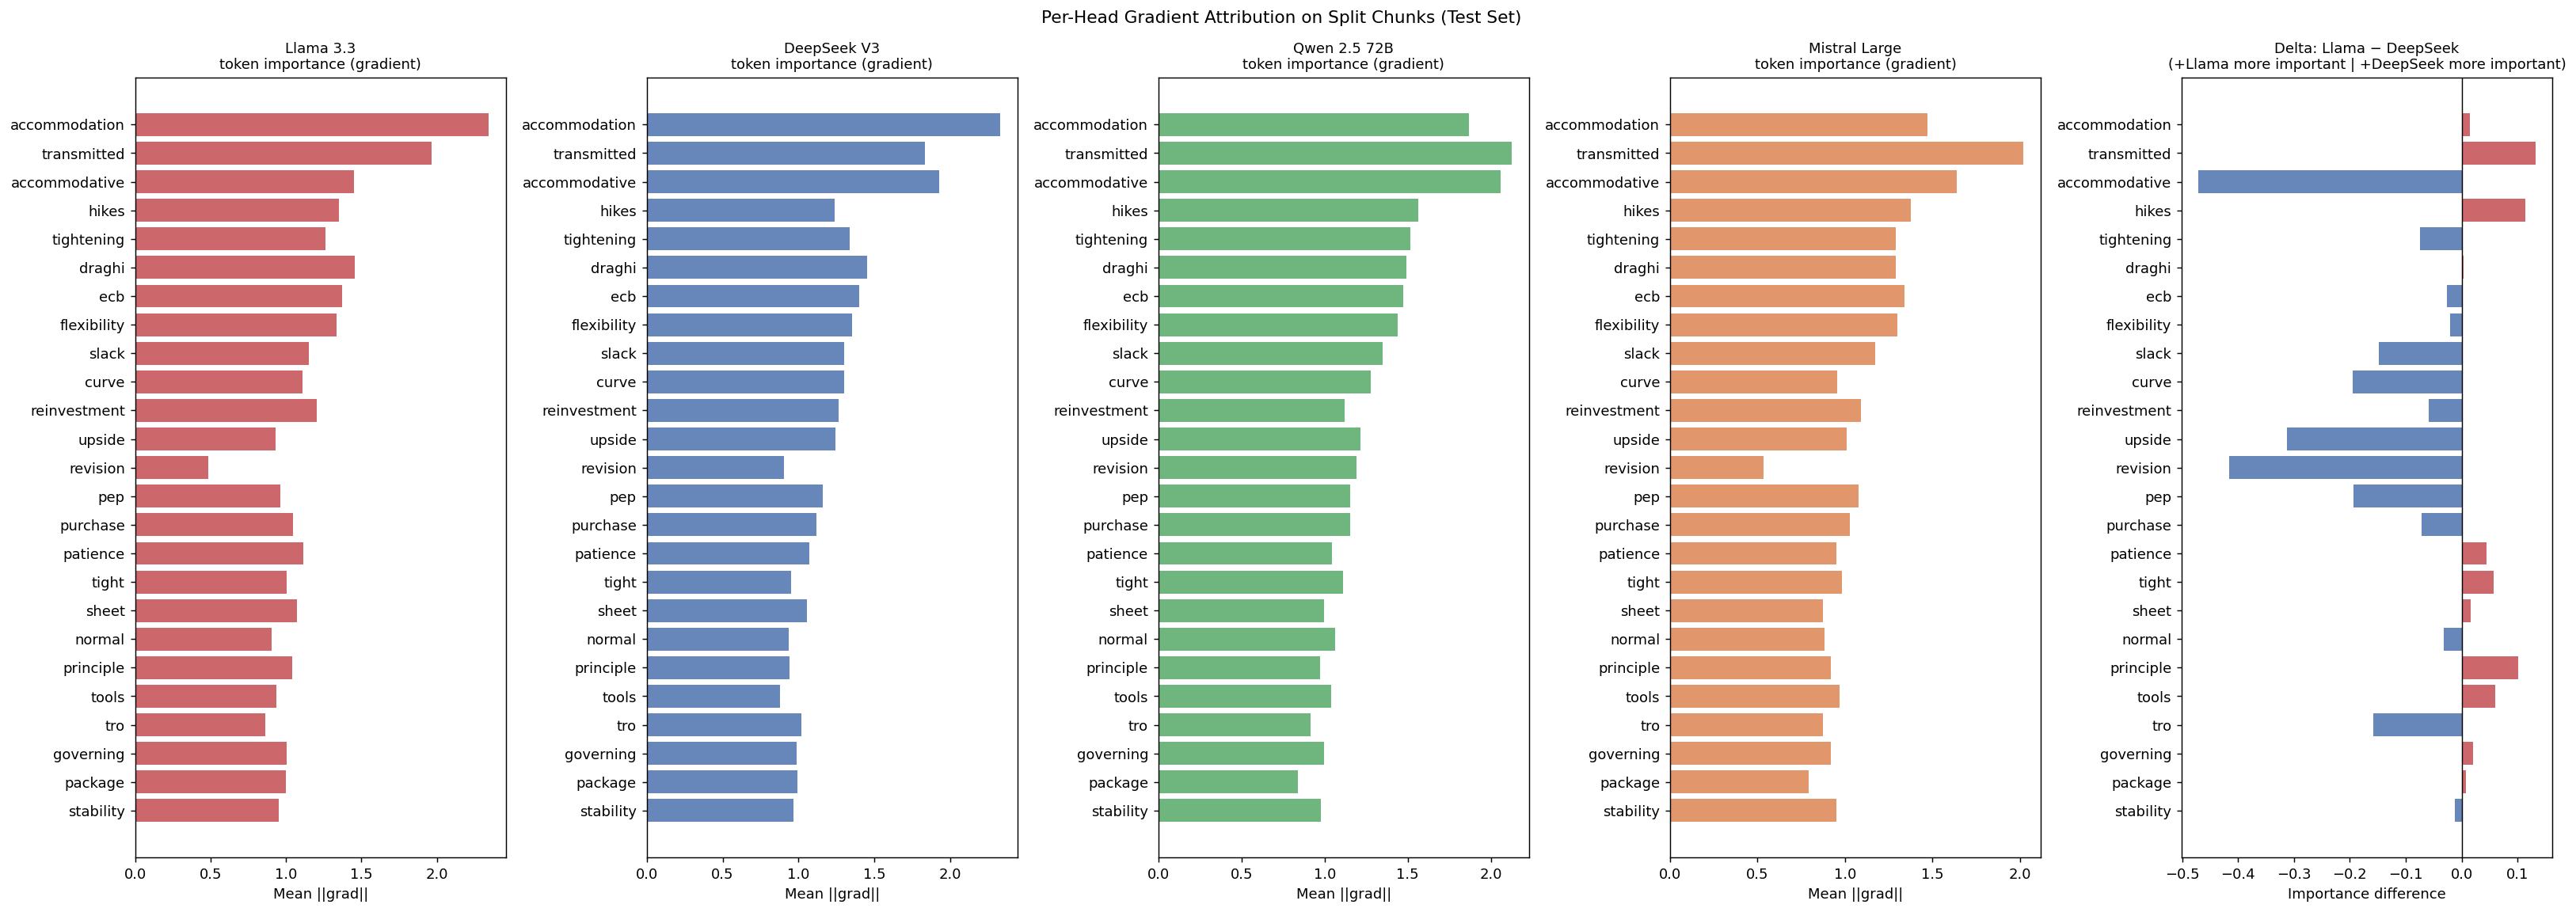
\includegraphics[width=\textwidth]{head_gradient_attribution.png}
  \caption{Per-head gradient attribution on disagreement chunks. The
           rightmost panel shows the Llama $-$ DeepSeek importance delta.
           Shared tokens appear in all panels at similar heights; entity
           tokens and directional tokens are the differentiators.}
\end{figure}

\subsection{Head weight cosine similarity: how similar are the decision rules?}

Each head is a $5 \times 768$ weight matrix. Flattening to a 3840-dimensional
vector and computing cosine similarity between all pairs tells us how similar
two models' learned decision rules are --- 1.0 would mean identical rules,
0 would mean orthogonal (unrelated) rules.

\begin{center}
\begin{tabular}{lc}
\toprule
\textbf{Pair} & \textbf{Cosine similarity} \\
\midrule
Llama 3.3 $\leftrightarrow$ Mistral Large   & \textbf{0.556} \\
Qwen 2.5 72B $\leftrightarrow$ Mistral Large & 0.520 \\
DeepSeek V3 $\leftrightarrow$ Qwen 2.5 72B  & 0.491 \\
DeepSeek V3 $\leftrightarrow$ Mistral Large  & 0.497 \\
Llama 3.3 $\leftrightarrow$ DeepSeek V3     & 0.486 \\
Llama 3.3 $\leftrightarrow$ Qwen 2.5 72B    & 0.485 \\
\bottomrule
\end{tabular}
\end{center}

All pairs are moderate and similar in range (0.49--0.56): no two heads learned
the same mapping, but none are orthogonal either. \textbf{Llama $\leftrightarrow$
Mistral is the most similar pair (0.556)}, recovering the empirical inter-rater
$\kappa$ structure without being given any information about pairwise agreement.

The PCA of the four head weight vectors (Figure~\ref{fig:head_weights})
reveals three structural clusters: Llama and Mistral sit close together
(right); Qwen is isolated far left (most structurally distinct, most
neutral-leaning); DeepSeek is isolated upward (different from all three
in a distinct direction, most label-unstable in CoT analysis).

\begin{figure}[h!]
  \centering
  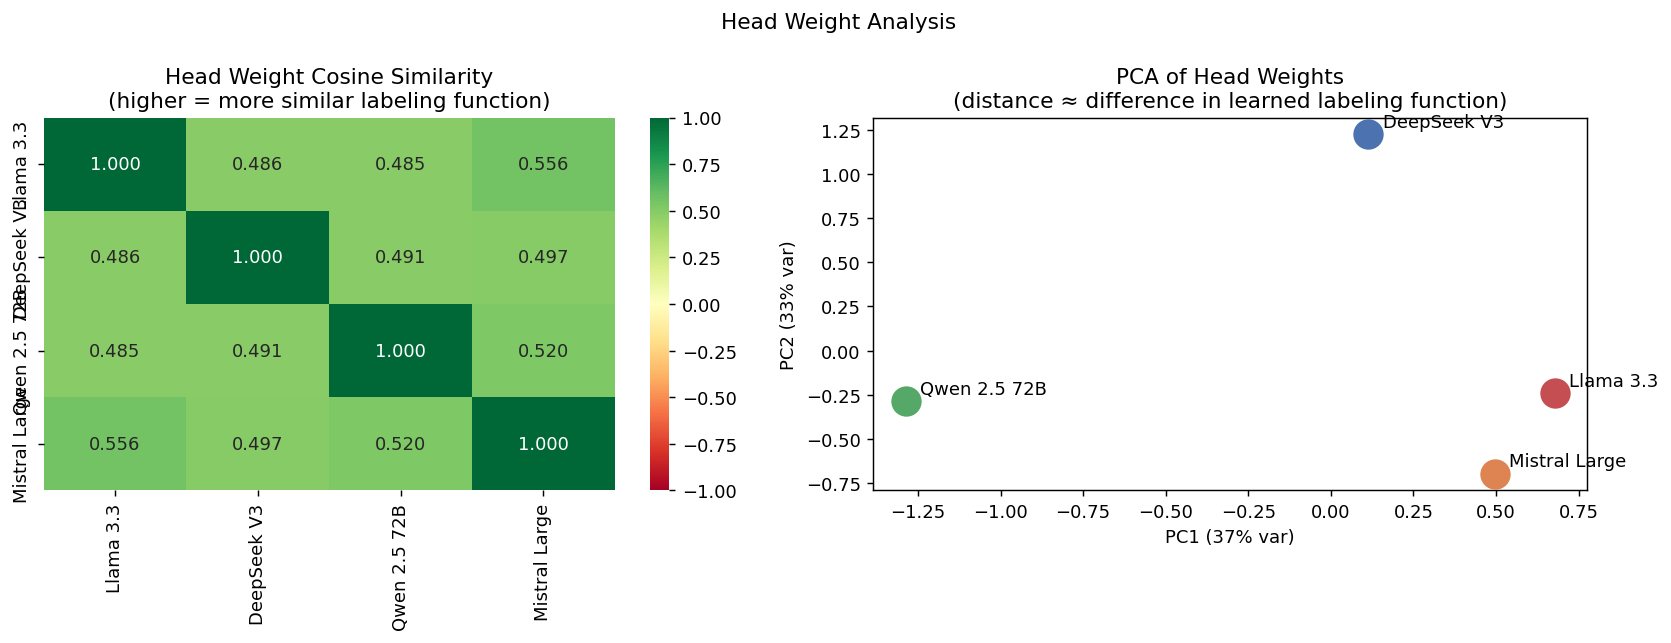
\includegraphics[width=\textwidth]{head_weight_similarity.png}
  \caption{Head weight cosine similarity (left) and PCA of head weight
           vectors (right). Llama and Mistral cluster; Qwen and DeepSeek
           are structural outliers in different directions.}
  \label{fig:head_weights}
\end{figure}

\subsection{Swap analysis: encoding vs.\ projection disagreement}

The final experiment asks: if we give all four heads the \emph{identical}
768-number summary of a disagreement chunk, do they still disagree?

\begin{center}
\begin{tabular}{lc}
\toprule
\textbf{Unique predictions across heads} & \textbf{Chunks (out of 194)} \\
\midrule
1 (all agree)   & \textbf{118 (60.8\%)} \\
2               & 71 (36.6\%) \\
3               & 4 \\
4 (all differ)  & 1 \\
\bottomrule
\end{tabular}
\end{center}

\textbf{60.8\% of disagreement chunks produce unanimous agreement from all
four heads when the encoding is shared.} This is the key decomposition result.
It means the majority of observed zero-shot disagreement came from each model
encoding the text differently --- different tokenisers, pretraining corpora,
and architectures produce different 768-number summaries, and those differences
propagate into different labels. When that variation is removed, disagreement
dissolves.

The remaining 39.2\% (76 chunks) is \emph{genuine} reaction-function
disagreement: same representation, different label.

Pairwise disagreement rates on the shared representation confirm the weight
similarity results:

\begin{center}
\begin{tabular}{lc}
\toprule
\textbf{Pair} & \textbf{Disagreement rate} \\
\midrule
Llama $\leftrightarrow$ Mistral   & \textbf{10.8\%} \\
DeepSeek $\leftrightarrow$ Qwen   & 19.1\% \\
Qwen $\leftrightarrow$ Mistral    & 23.2\% \\
Llama $\leftrightarrow$ DeepSeek  & 28.4\% \\
Llama $\leftrightarrow$ Qwen      & 29.4\% \\
DeepSeek $\leftrightarrow$ Mistral & \textbf{32.0\%} \\
\bottomrule
\end{tabular}
\end{center}

Llama--Mistral disagree on only 10.8\% of disagreement chunks when sharing
an encoder --- their decision rules are nearly identical. DeepSeek--Mistral
disagree most (32.0\%), consistent with DeepSeek's structural isolation in PCA.

\begin{figure}[h!]
  \centering
  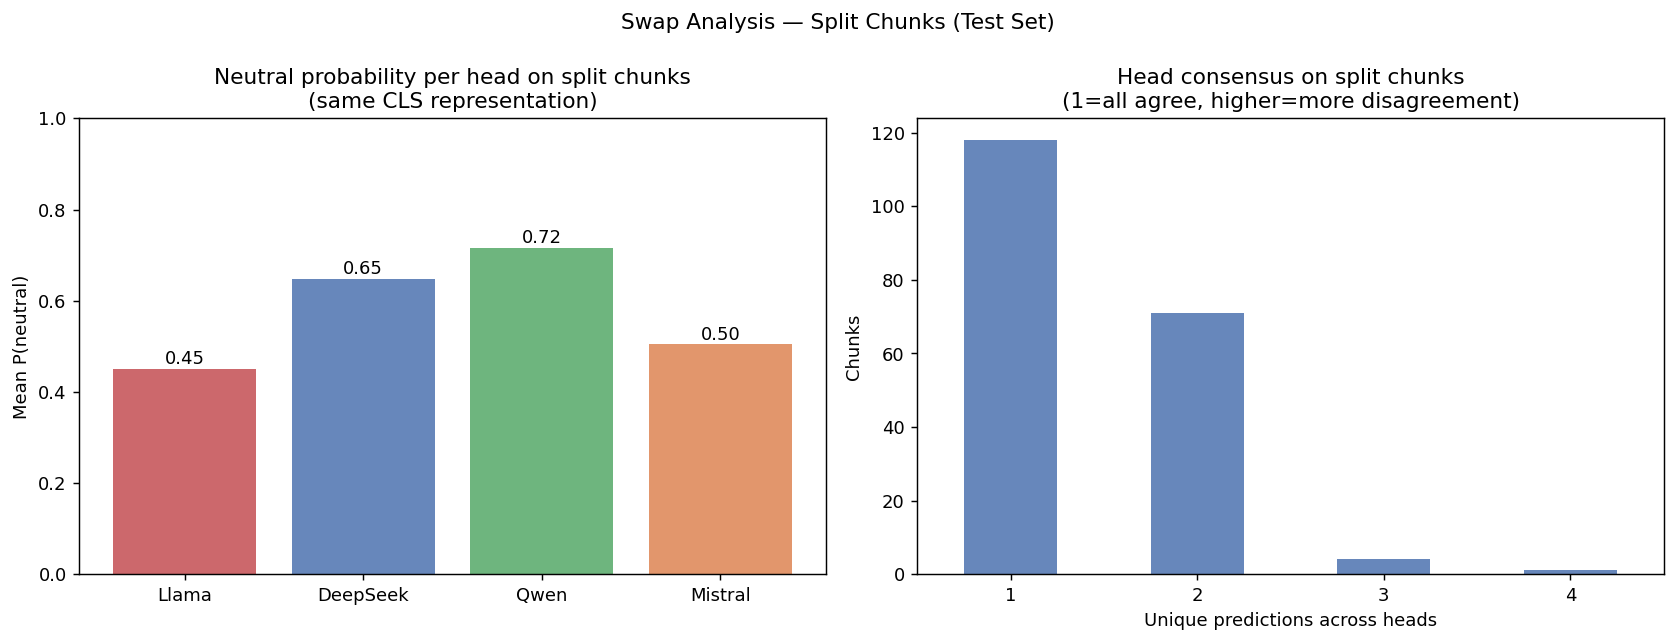
\includegraphics[width=\textwidth]{swap_analysis_multihead.png}
  \caption{Swap analysis. \textit{Left:} mean P(neutral) per head on
           disagreement chunks (same CLS representation) --- Llama is most
           directional, Qwen most conservative. \textit{Right:} head consensus
           distribution --- 60.8\% of chunks get unanimous agreement.}
\end{figure}

% ─────────────────────────────────────────────────────────────────────────────
\section{Main Finding and Implications}

\subsection{The central result}

\begin{center}
\fbox{\parbox{0.88\textwidth}{%
\textbf{All four LLMs perceive the same signals in central bank text.
Disagreement arises because each model applies a different linear projection
from signal representation to stance label --- a learned reaction function,
not a perceptual difference.}
}}
\end{center}

To use the thesis's own language: the models have all read the same economic
data (the text), but they apply different Taylor rules to it. The disagreement
is in the rule, not the data.

The net hawk timeseries (Figure~\ref{fig:timeseries}) shows what this looks
like empirically: the four models trace similar trends (same direction over
time) but with systematic offsets driven by their different neutral thresholds.

\begin{figure}[h!]
  \centering
  \includegraphics[width=\textwidth]{timeseries_net_hawk_llama33_deepseekv3_qwen25_72b_mistrallarge_or.png}
  \caption{Net hawk score per model per bank over time. Models agree on
           trend direction but differ on level, reflecting different
           neutral-probability thresholds.}
  \label{fig:timeseries}
\end{figure}

\subsection{Implications for RQ1 and RQ2}

\textbf{RQ1} (do LLMs disagree, where?): Yes. The disagreement is systematic,
localised to specific spans, and driven by (a) different neutral thresholds
and (b) entity-sensitivity in Llama and DeepSeek. It is not noise.

\textbf{RQ2} (does LLM choice affect shock estimates?): Yes, in two ways.
First, the level of estimated hawkishness depends on which model's neutral
threshold is used --- Qwen and DeepSeek produce more neutral labels overall.
Second, for cross-bank comparisons, Llama and DeepSeek are contaminated by
speaker-identity cues (\textit{draghi}, \textit{ecb}); Qwen and Mistral are
more purely lexical and may be preferable for that use case. Ensembling
across all four models reduces both biases.

\textbf{Flag on DeepSeek:} Its structural isolation in PCA, low chain-of-thought
label stability (20\% vs.\ 58\% for Llama), and highest phrase-masking
self-calibration rate all suggest its zero-shot labels carry more noise than
the other three. Results should be reported with and without DeepSeek.

\subsection{Next steps: RQ3 and RQ4}

The VAR estimation (cross-bank shock propagation, RQ3) and the asymmetric
market reaction analysis (RQ4) will use the ensemble score as the baseline
stance measure and include model-choice robustness checks as a sensitivity
analysis, flagging any result that is sensitive to which LLM is used.

% ─────────────────────────────────────────────────────────────────────────────
\section*{Note on Figures}
All timeseries and agreement figures are generated by
\path{notebooks/13_stance_timeseries.ipynb}. The gradient attribution,
head weight, and swap analysis figures are outputs of
\path{notebooks/multihead_stance_colab.ipynb} (Colab, T4~GPU).
Full methodology and literature references: \path{notes/multihead_analysis_summary.md}.

\end{document}
